% =====================================================================
%  Eigene Fotos der Dübelfräse im FabLab mit nummerierten Bedienelementen.
%  Koordinaten relativ zum jeweiligen Foto: (0,0) unten links, (1,1) oben rechts.
%  Nummern wie in der Tabelle in einweisung_Duebelfraese.tex
% =====================================================================
% \fotonr{Nummer}{Position der Nummer}{Bauteil}, nur innerhalb eines Foto-Scopes
\newcommand{\fotonr}[3]{%
  \draw[white, line width=2pt, line cap=round] (#2) -- (#3);
  \draw[black, line width=0.8pt] (#2) -- (#3);
  \fill[black] (#3) circle[radius=0.7mm];
  \node[marke, minimum size=5.5mm, font=\small\bfseries, line width=1pt] at (#2) {#1};}
\newcommand{\fototitel}[1]{\node[anchor=north west, fill=white, fill opacity=0.85,
  text opacity=1, font=\small\bfseries, inner sep=1.2mm] at (0,1) {#1};}

\begin{tikzpicture}
  \node[anchor=south west, inner sep=0pt] (a) at (0,0)
    {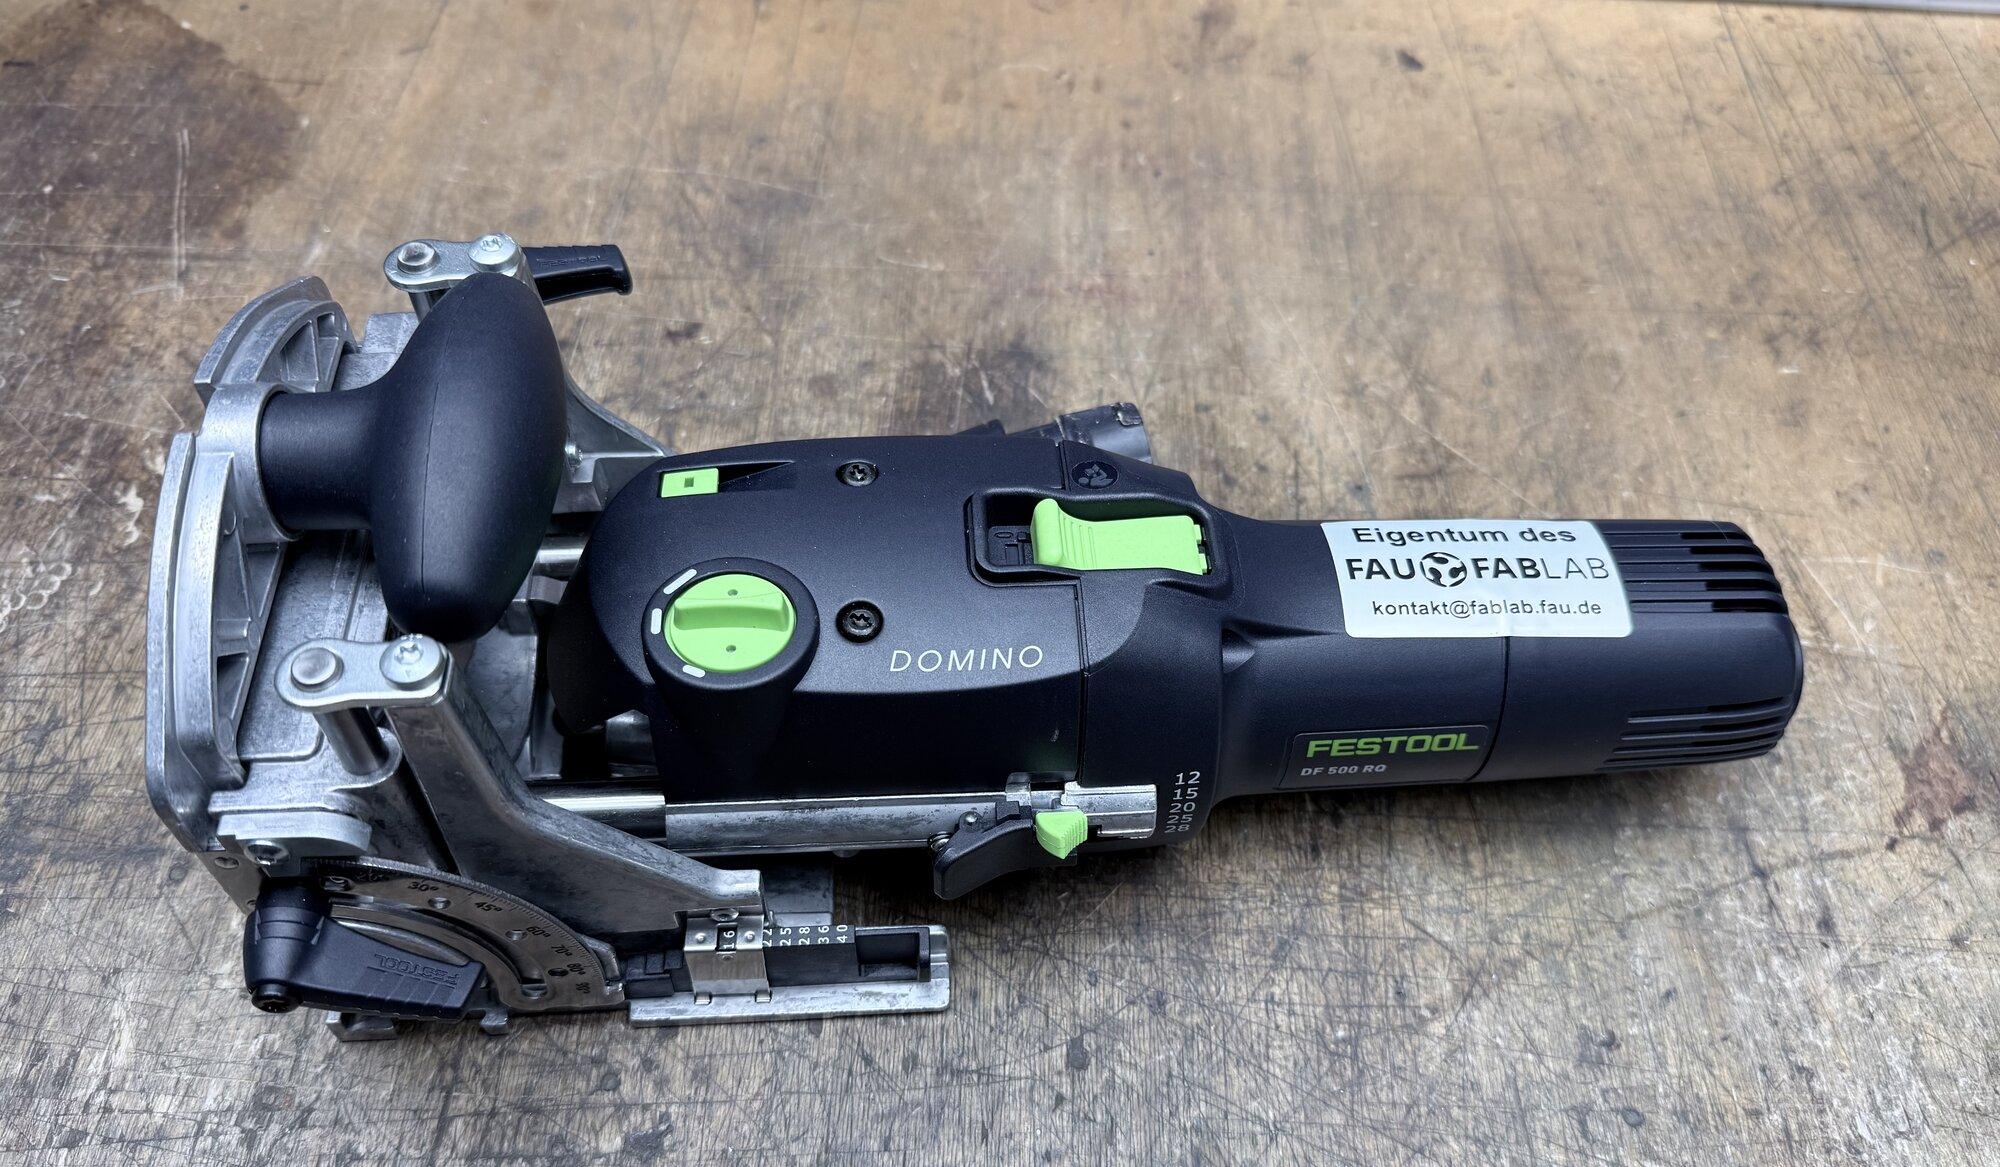
\includegraphics[width=\textwidth]{bilder/domino-oben.jpg}};
  \begin{scope}[x={(a.south east)}, y={(a.north west)}]
    \fotonr{1}{0.60,0.82}{0.557,0.543}
    \fotonr{2}{0.93,0.80}{0.88,0.55}
    \fotonr{3}{0.12,0.88}{0.219,0.613}
    \fotonr{4}{0.38,0.85}{0.365,0.468}
    \fotonr{5}{0.56,0.10}{0.529,0.292}
    \fotonr{6}{0.07,0.12}{0.183,0.253}
  \end{scope}
\end{tikzpicture}

\vspace{2mm}
\begin{tikzpicture}
  \node[anchor=south west, inner sep=0pt] (b) at (0,0)
    {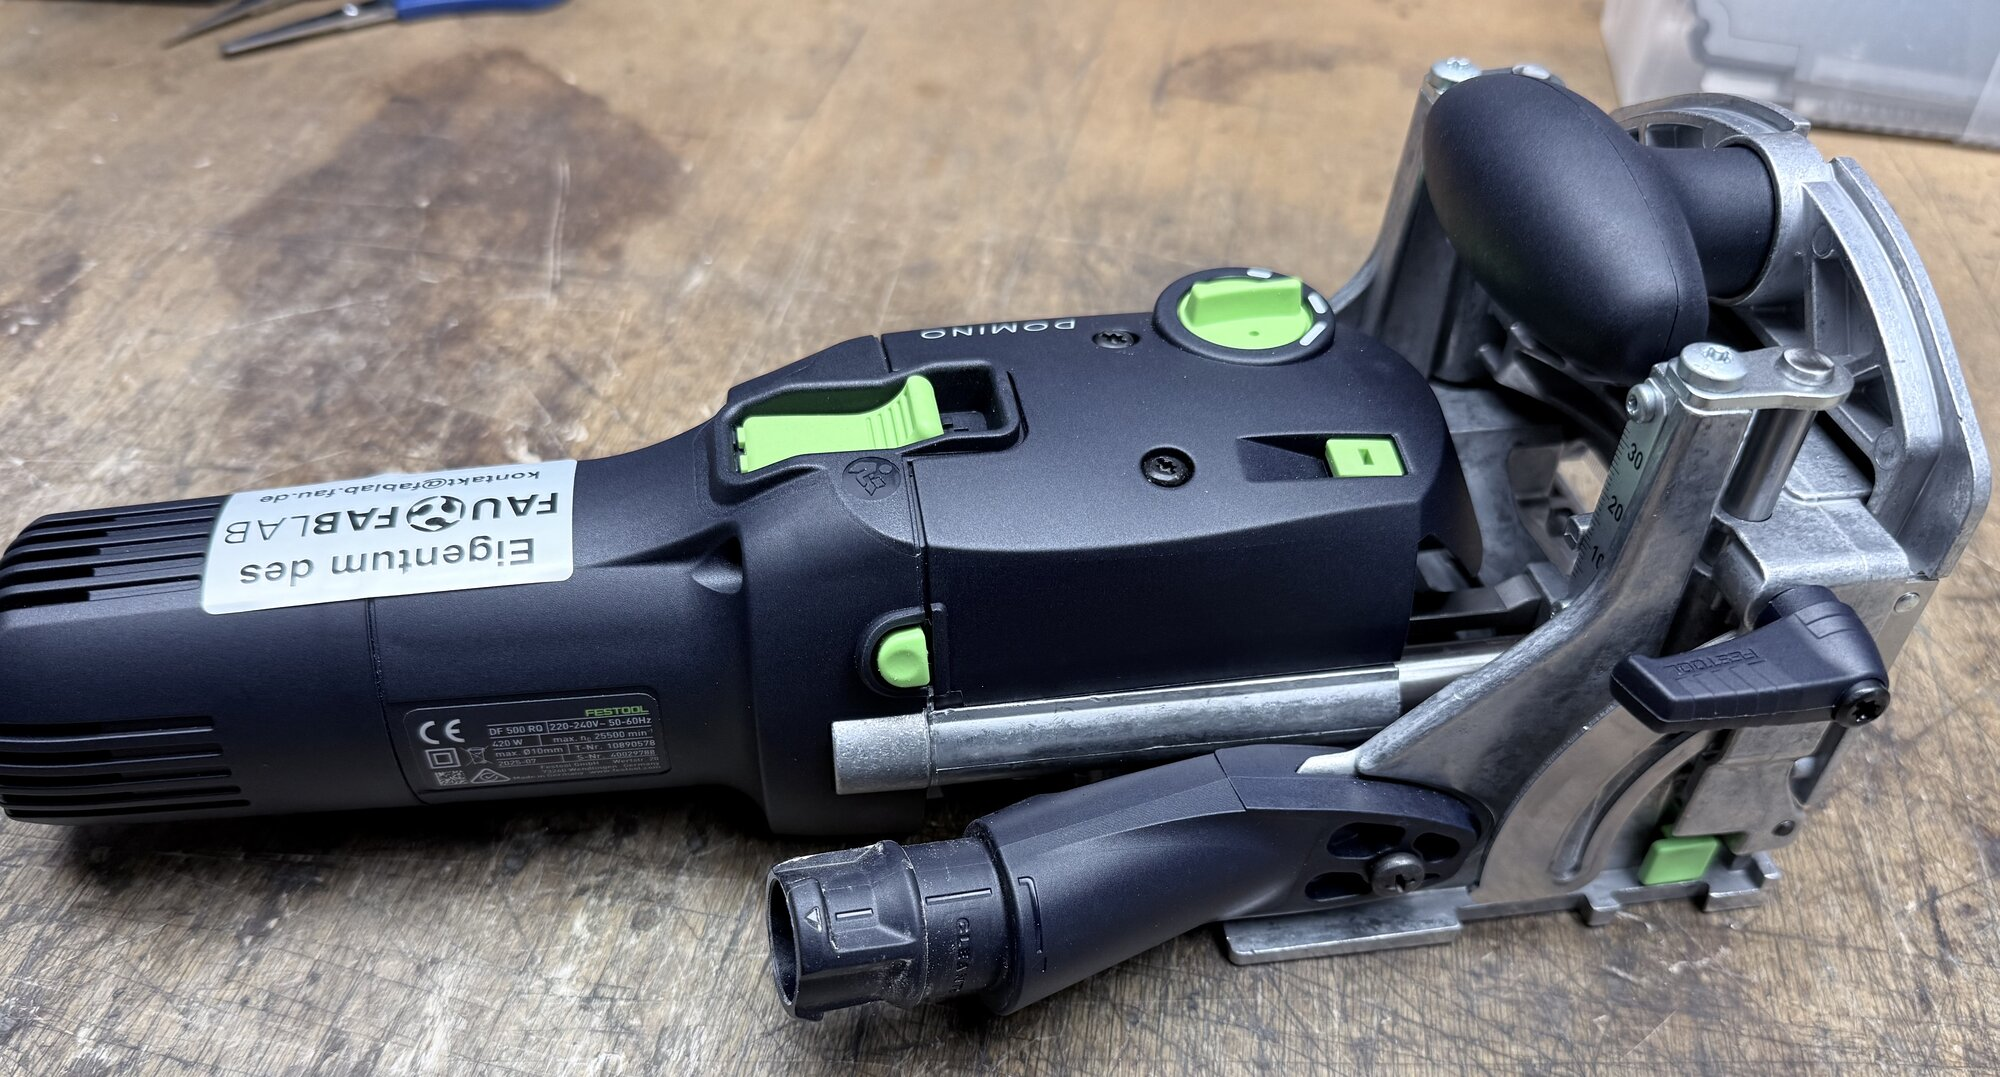
\includegraphics[width=0.6\textwidth]{bilder/domino-seite.jpg}};
  \node[anchor=south west, inner sep=0pt] (c) at ([xshift=0.02\textwidth]b.south east)
    {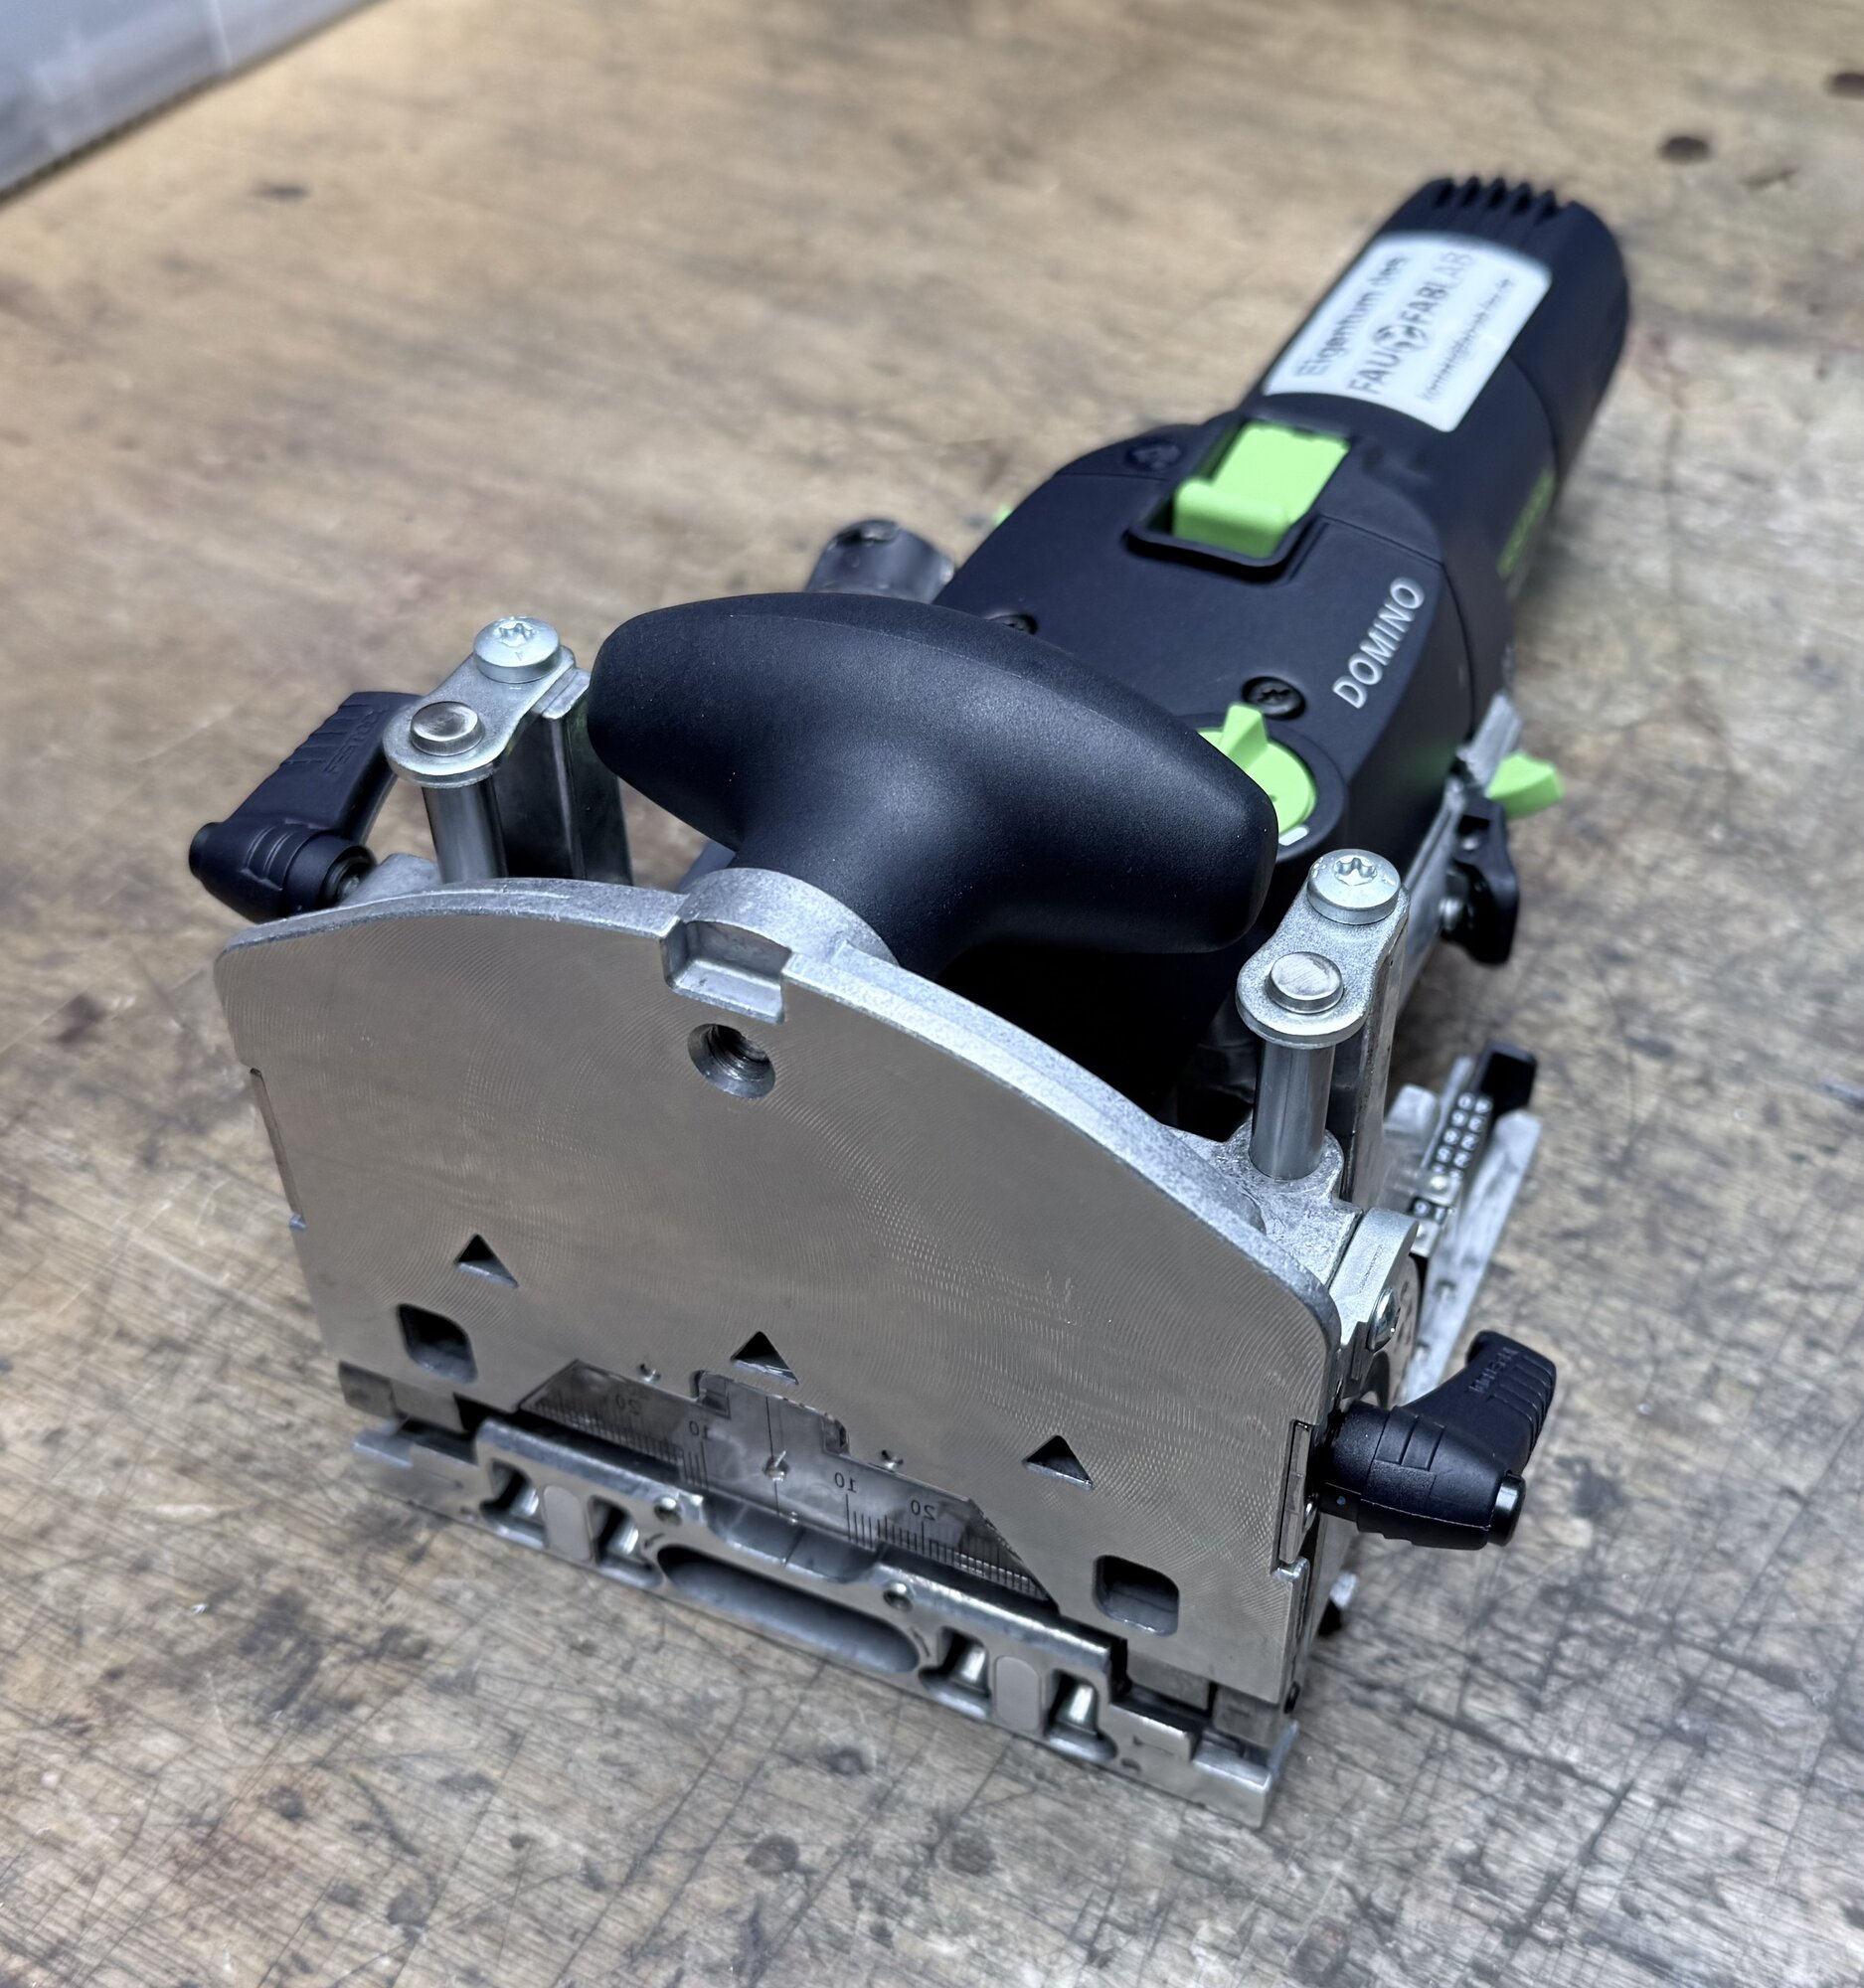
\includegraphics[height=0.3229\textwidth]{bilder/domino-vorn.jpg}};
  \begin{scope}[x={(b.south east)}, y={(b.north west)}]
    \fotonr{7}{0.70,0.88}{0.802,0.525}
    \fotonr{8}{0.95,0.18}{0.858,0.389}
    \fotonr{9}{0.20,0.12}{0.414,0.139}
  \end{scope}
  \begin{scope}[shift={(c.south west)}, x={($(c.south east)-(c.south west)$)}, y={($(c.north west)-(c.south west)$)}]
    \fotonr{10}{0.14,0.14}{0.406,0.323}
  \end{scope}
\end{tikzpicture}
